\begin{tikzpicture}

\tikzset{
    >={Latex[width=2mm,length=2mm]},
    base/.style = {rectangle, rounded corners=1pt, draw=black,
                   minimum width=4.5cm, minimum height=2.25cm,
                   text centered},
    blockstyle/.style = {base, fill=gray!10}
}

%% POMDP loop
\node[blockstyle, rounded corners=25pt, dashed, fill=gray!5, minimum width=20cm, minimum height=6cm] at (0,-0.6) (pomdp) {};

\node[above=10pt of pomdp.south west, anchor=west, xshift=10mm, font=\large] {batched belief-state planning (POMDP)};
\node[below=10pt of pomdp.south west, anchor=west, xshift=10mm, font=\large\color{gray}] {chapter \ref{ch:bbmdp}};


%% Planner
\node[blockstyle] (planner) at (0,0) {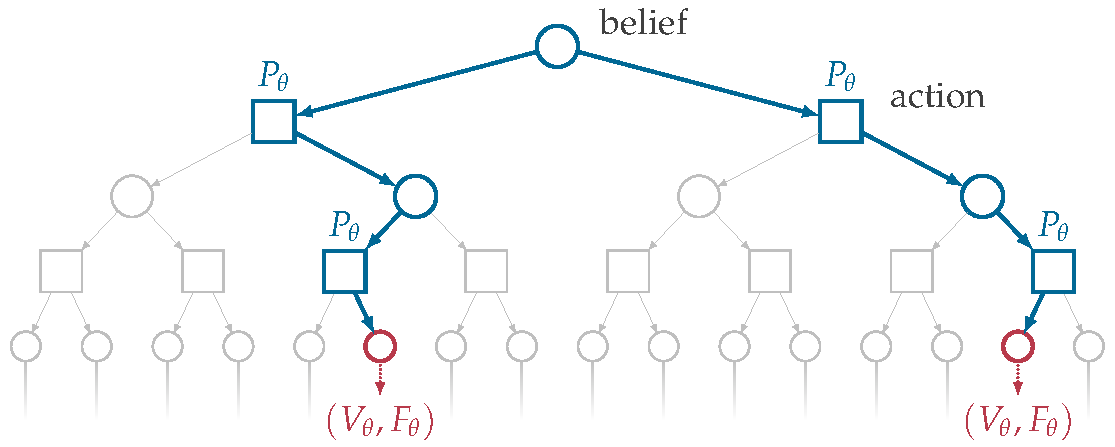
\includegraphics[width=4cm]{diagrams/introduction/tree-search.pdf}};

\node[above=2pt of planner.north, anchor=south, font=\Large] {safe planner};
\node[below=2pt of planner.south, anchor=north, font=\large\color{gray}] {chapters \ref{ch:betazero} and \ref{ch:constrainedzero}};


%% Belief updater
\node[blockstyle, left=2cm of planner] (belief) {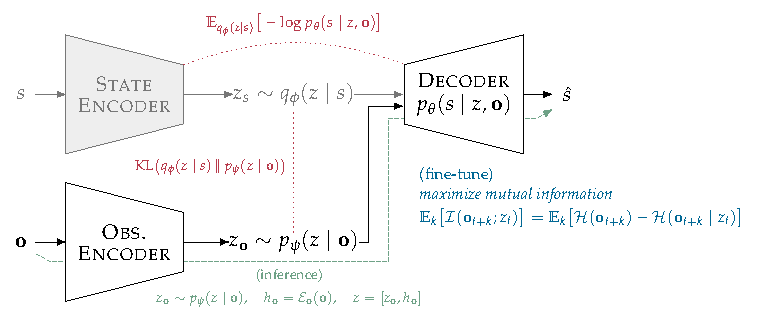
\includegraphics[width=3.75cm]{diagrams/introduction/ivae.pdf}};

\node[above=2pt of belief.north, anchor=south, font=\Large] {belief updater};
\node[below=2pt of belief.south, anchor=north, font=\large\color{gray}] {chapter \ref{ch:ivae}};


%% Environment
\node[blockstyle, right=2cm of planner] (env) {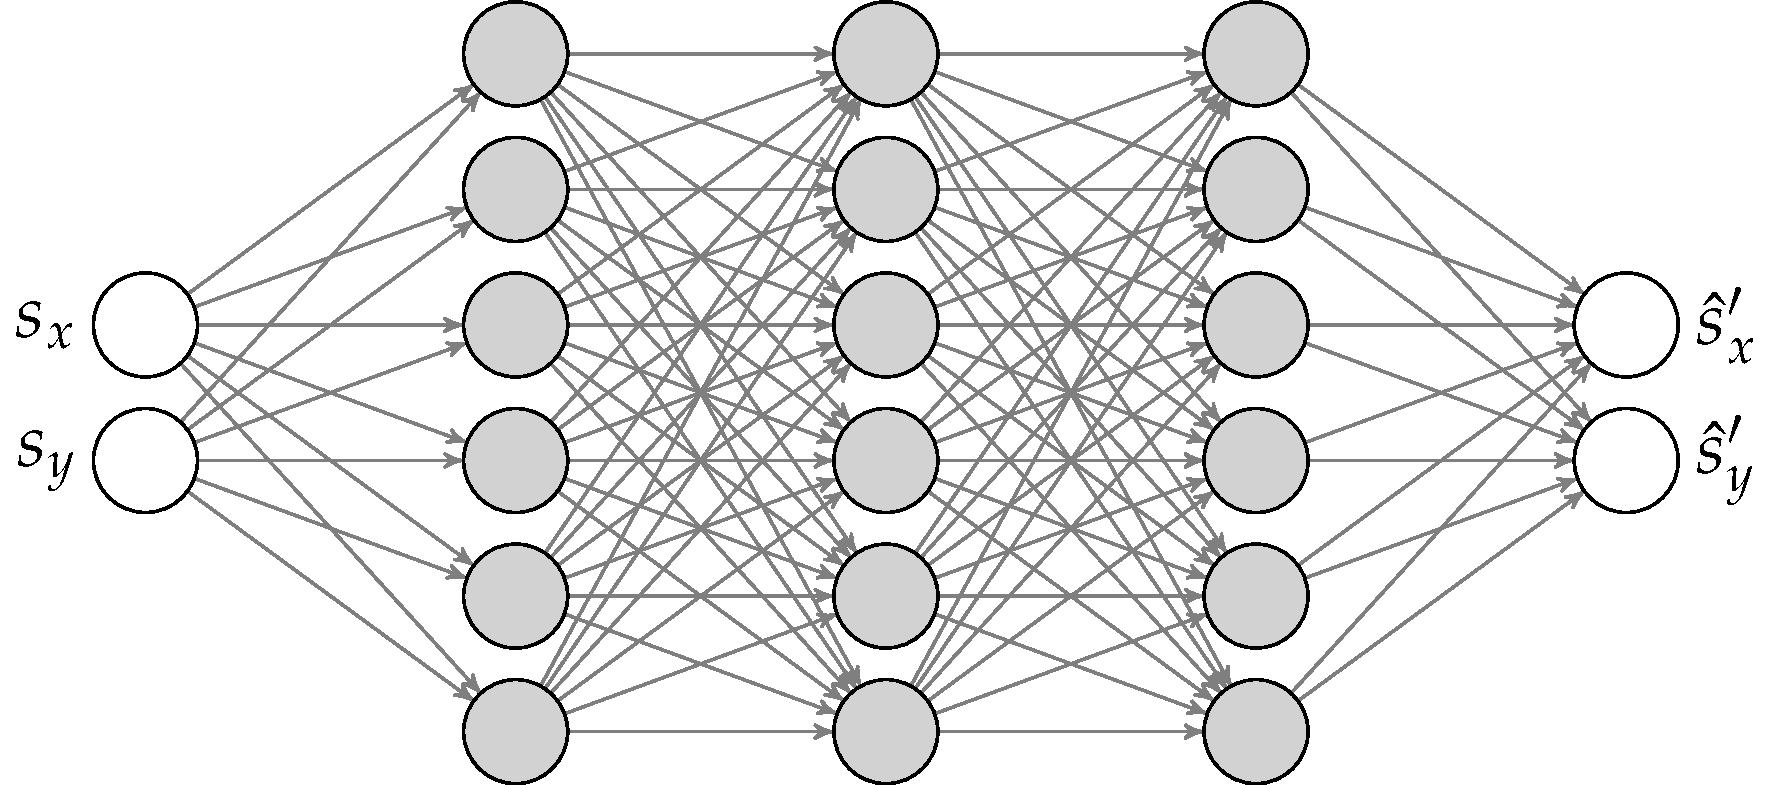
\includegraphics[width=3cm]{diagrams/introduction/env.pdf}};

\node[above=2pt of env.north, anchor=south, font=\Large] {environment};
\node[below=2pt of env.south, anchor=north, font=\large\color{gray}] {chapter \ref{ch:future} (future work)};


%% Bayesian safety validation
\node[blockstyle, rounded corners=25pt, fill=none, minimum width=22cm, minimum height=8cm] at (0,-0.6) (bsv) {};

\node[fill=none, draw=none, anchor=east, font=\large] (input) at ($(bsv.west)+(-7mm,0)$) {\shortstack{adversarial\\input}};
\node[fill=none, draw=none, anchor=west, font=\large] (output) at ($(bsv.east)+(7mm,0)$) {\shortstack{failure\\output}};


%% Arrows
\draw[->, font=\large] (belief) -- (planner) node[midway, above] {belief} node[midway, below] {$b_t$};

\draw[->, font=\large] (planner) -- (env) node[midway, above] {action} node[midway, below] {$a_t$};

\draw[->, font=\large] ($(env.south)-(0,7mm)$) to[out=230, in=310, looseness=0.28] node[midway, above, sloped] {observation} node[midway, below, sloped] {$o_t$} ($(belief.south)-(0,7mm)$);

\draw[->] (input) -- (bsv);
\draw[->] (bsv) -- (output);

\def\offset{6cm}

\draw[->, rounded corners=10pt]
  (output.south)
  -- ++(0,-\offset)
  -- node[blockstyle, midway] (gp) {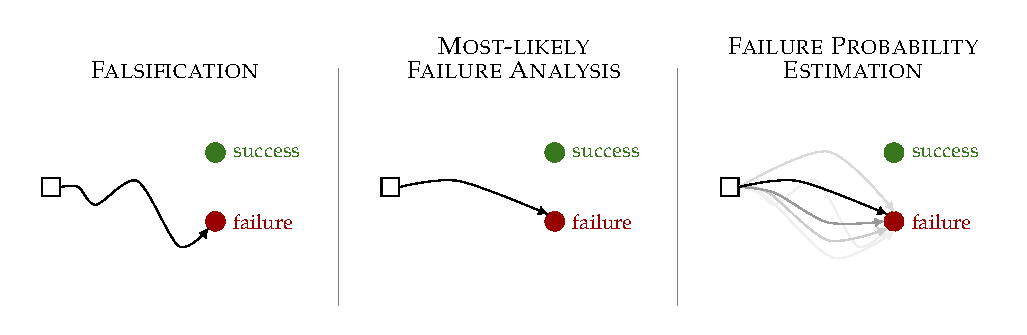
\includegraphics[width=4.5cm]{diagrams/introduction/safety-validation.pdf}} ($(input.south)+(0,-\offset)$)
  -- (input.south);

\node[above=2pt of gp.north, anchor=south, font=\Large] {black-box safety validation};
\node[below=2pt of gp.south, anchor=north, font=\large\color{gray}] {chapter \ref{ch:bsv}};

\end{tikzpicture}